%<dscrpt>Fichier de déclarations Latex à inclure au début d'un élément de cours.</dscrpt>

\documentclass[a4paper]{article}
\usepackage[hmargin={1.8cm,1.8cm},vmargin={2.4cm,2.4cm},headheight=13.1pt]{geometry}

%includeheadfoot,scale=1.1,centering,hoffset=-0.5cm,
\usepackage[pdftex]{graphicx,color}
\usepackage[french]{babel}
%\selectlanguage{french}
\addto\captionsfrench{
  \def\contentsname{Plan}
}
\usepackage{fancyhdr}
\usepackage{floatflt}
\usepackage{amsmath}
\usepackage{amssymb}
\usepackage{amsthm}
\usepackage{stmaryrd}
%\usepackage{ucs}
\usepackage[utf8]{inputenc}
%\usepackage[latin1]{inputenc}
\usepackage[T1]{fontenc}


\usepackage{titletoc}
%\contentsmargin{2.55em}
\dottedcontents{section}[2.5em]{}{1.8em}{1pc}
\dottedcontents{subsection}[3.5em]{}{1.2em}{1pc}
\dottedcontents{subsubsection}[5em]{}{1em}{1pc}

\usepackage[pdftex,colorlinks={true},urlcolor={blue},pdfauthor={remy Nicolai},bookmarks={true}]{hyperref}
\usepackage{makeidx}

\usepackage{multicol}
\usepackage{multirow}
\usepackage{wrapfig}
\usepackage{array}
\usepackage{subfig}


%\usepackage{tikz}
%\usetikzlibrary{calc, shapes, backgrounds}
%pour la présentation du pseudo-code
% !!!!!!!!!!!!!!      le package n'est pas présent sur le serveur sous fedora 16 !!!!!!!!!!!!!!!!!!!!!!!!
%\usepackage[french,ruled,vlined]{algorithm2e}

%pr{\'e}sentation du compteur de niveau 2 dans les listes
\makeatletter
\renewcommand{\labelenumii}{\theenumii.}
\renewcommand{\thesection}{\Roman{section}.}
\renewcommand{\thesubsection}{\arabic{subsection}.}
\renewcommand{\thesubsubsection}{\arabic{subsubsection}.}
\makeatother


%dimension des pages, en-t{\^e}te et bas de page
%\pdfpagewidth=20cm
%\pdfpageheight=14cm
%   \setlength{\oddsidemargin}{-2cm}
%   \setlength{\voffset}{-1.5cm}
%   \setlength{\textheight}{12cm}
%   \setlength{\textwidth}{25.2cm}
   \columnsep=1cm
   \columnseprule=0.5pt

%En tete et pied de page
\pagestyle{fancy}
\lhead{MPSI-\'Eléments de cours}
\rhead{\today}
%\rhead{25/11/05}
\lfoot{\tiny{Cette création est mise à disposition selon le Contrat\\ Paternité-Pas d'utilisations commerciale-Partage des Conditions Initiales à l'Identique 2.0 France\\ disponible en ligne http://creativecommons.org/licenses/by-nc-sa/2.0/fr/
} }
\rfoot{\tiny{Rémy Nicolai \jobname}}


\newcommand{\baseurl}{http://back.maquisdoc.net/data/cours\_nicolair/}
\newcommand{\urlexo}{http://back.maquisdoc.net/data/exos_nicolair/}
\newcommand{\urlcours}{https://maquisdoc-math.fra1.digitaloceanspaces.com/}

\newcommand{\N}{\mathbb{N}}
\newcommand{\Z}{\mathbb{Z}}
\newcommand{\C}{\mathbb{C}}
\newcommand{\R}{\mathbb{R}}
\newcommand{\D}{\mathbb{D}}
\newcommand{\K}{\mathbf{K}}
\newcommand{\Q}{\mathbb{Q}}
\newcommand{\F}{\mathbf{F}}
\newcommand{\U}{\mathbb{U}}
\newcommand{\p}{\mathbb{P}}


\newcommand{\card}{\mathop{\mathrm{Card}}}
\newcommand{\Id}{\mathop{\mathrm{Id}}}
\newcommand{\Ker}{\mathop{\mathrm{Ker}}}
\newcommand{\Vect}{\mathop{\mathrm{Vect}}}
\newcommand{\cotg}{\mathop{\mathrm{cotan}}}
\newcommand{\sh}{\mathop{\mathrm{sh}}}
\newcommand{\ch}{\mathop{\mathrm{ch}}}
\newcommand{\argsh}{\mathop{\mathrm{argsh}}}
\newcommand{\argch}{\mathop{\mathrm{argch}}}
\newcommand{\tr}{\mathop{\mathrm{tr}}}
\newcommand{\rg}{\mathop{\mathrm{rg}}}
\newcommand{\rang}{\mathop{\mathrm{rg}}}
\newcommand{\Mat}{\mathop{\mathrm{Mat}}}
\newcommand{\MatB}[2]{\mathop{\mathrm{Mat}}_{\mathcal{#1}}\left( #2\right) }
\newcommand{\MatBB}[3]{\mathop{\mathrm{Mat}}_{\mathcal{#1} \mathcal{#2}}\left( #3\right) }
\renewcommand{\Re}{\mathop{\mathrm{Re}}}
\renewcommand{\Im}{\mathop{\mathrm{Im}}}
\renewcommand{\th}{\mathop{\mathrm{th}}}
\newcommand{\repere}{$(O,\overrightarrow{i},\overrightarrow{j},\overrightarrow{k})$}
\newcommand{\cov}{\mathop{\mathrm{Cov}}}

\newcommand{\absolue}[1]{\left| #1 \right|}
\newcommand{\fonc}[5]{#1 : \begin{cases}#2 \rightarrow #3 \\ #4 \mapsto #5 \end{cases}}
\newcommand{\depar}[2]{\dfrac{\partial #1}{\partial #2}}
\newcommand{\norme}[1]{\left\| #1 \right\|}
\newcommand{\se}{\geq}
\newcommand{\ie}{\leq}
\newcommand{\trans}{\mathstrut^t\!}
\newcommand{\val}{\mathop{\mathrm{val}}}
\newcommand{\grad}{\mathop{\overrightarrow{\mathrm{grad}}}}

\newtheorem*{thm}{Théorème}
\newtheorem{thmn}{Théorème}
\newtheorem*{prop}{Proposition}
\newtheorem{propn}{Proposition}
\newtheorem*{pa}{Présentation axiomatique}
\newtheorem*{propdef}{Proposition - Définition}
\newtheorem*{lem}{Lemme}
\newtheorem{lemn}{Lemme}

\theoremstyle{definition}
\newtheorem*{defi}{Définition}
\newtheorem*{nota}{Notation}
\newtheorem*{exple}{Exemple}
\newtheorem*{exples}{Exemples}


\newenvironment{demo}{\renewcommand{\proofname}{Preuve}\begin{proof}}{\end{proof}}
%\renewcommand{\proofname}{Preuve} doit etre après le begin{document} pour fonctionner

\theoremstyle{remark}
\newtheorem*{rem}{Remarque}
\newtheorem*{rems}{Remarques}

\renewcommand{\indexspace}{}
\renewenvironment{theindex}
  {\section*{Index} %\addcontentsline{toc}{section}{\protect\numberline{0.}{Index}}
   \begin{multicols}{2}
    \begin{itemize}}
  {\end{itemize} \end{multicols}}


%pour annuler les commandes beamer
\renewenvironment{frame}{}{}
\newcommand{\frametitle}[1]{}
\newcommand{\framesubtitle}[1]{}

\newcommand{\debutcours}[2]{
  \chead{#1}
  \begin{center}
     \begin{huge}\textbf{#1}\end{huge}
     \begin{Large}\begin{center}Rédaction incomplète. Version #2\end{center}\end{Large}
  \end{center}
  %\section*{Plan et Index}
  %\begin{frame}  commande beamer
  \tableofcontents
  %\end{frame}   commande beamer
  \printindex
}


\makeindex
\begin{document}
\noindent

\debutcours{Courbes planes paramétrées}{alpha}

L'étude des courbes sera reprise en fin d'année en particulier pour l'introduction des propriétés métriques et la classification locale.\newline
Cette section utilise les définitions et résultats relatifs aux \href{\baseurl C4199.pdf}{Fonctions d'une variable réelle et à valeurs vectorielles} du Glossaire de début d'année.
\section{Vocabulaire}
courbe paramétrée, fonction, mouvement, vitesse, accélération.

courbe plane (ensemble de points), trajectoire ou support d'une courbe paramétrée. Des courbes plus générales que les graphes.\newline
changements de paramètres, paramétrages admissibles\newline
exemples de types de paramétrisation : $(x(t),y(t)$, $(x,y(x))$, $(x(y),y)$, $\rho(\theta)\overrightarrow{e}_\theta$, $\rho(t)\overrightarrow{e}_\theta(t)$, mouvement à accélération centrale\index{courbe paramétrée à accélération centrale}, mouvement uniforme (= paramétrisation normale), ....

\section{\'Etude locale}
\subsection{Tangente, normale}
Point régulier\index{point régulier}: vitesse, tangente, normale. Point stationnaire. Point birégulier\index{point birégulier}.
\begin{figure}[!ht]
 \centering
 \input{C6430_1.pdf_t}
 \caption{Définition de la tangente}
\end{figure}
\begin{defi}[Essai de définition d'une tangente]\index{tangente}
 La courbe paramétrée $f$ admet un tangente au point $f(t_0)$ lorsque 
\begin{displaymath}
 t \rightarrow \dfrac{\overrightarrow{f(t_0)f(t)}}{\Vert \overrightarrow{f(t_0)f(t)}\Vert}
\end{displaymath}
converge à droite et à gauche (strictement) de $t_0$ vers des vecteurs colinéaires. La tangente en $t_0$ est alors la droite qui passe par $f(t_0)$ et de direction la droite vectorielle engendrée par ces vecteurs. Lorsque il y a convergence mais vers des vecteurs différents, on dira que la courbe admet des demi-tangentes. 
\end{defi}

\begin{prop}
 Une courbe paramétrée $f$ admet en un point régulier $f(t_0)$ une tangente dirigée par $\overrightarrow{f}^\prime(t_0)$.
\end{prop}

La normale\index{normale} est la droite perpendiculaire à la tangente en $f(t_0)$.
\'Equations de la tangente et de la normale en un point régulier.

\subsection{Position par rapport à la tangente et à la normale}
Demi-plans définis par les équations de la tangente et de la normale.
\index{qc: forme locale de la courbe (cas birégulier)}
Point birégulier : accélération, position locale de la courbe par rapport à la tangente et à la normale.
\begin{figure}[!ht]
 \centering
 \input{C6430_2.pdf_t}
 \caption{Point birégulier. Position par rapport à la normale et à la tangente}
\end{figure}


La classification en  point normal, d'inflexion, de rebroussement (de première ou de deuxième espèce) ne sera exposée qu'en fin d'année.
\index{qc: vitesse et accélération dans le repère polaire}
Calculs de vitesse pour $\rho(\theta)\overrightarrow{e}_\theta$ ou  $\rho(t)\overrightarrow{e}_\theta(t)$

\subsection{\'Etude locale : branches infinies}
\index{qc: direction asymptotique et asymptote}
Remarques sur les définitions possibles de la notion de branches infinie\index{branche infinie}. On se limite à un cas particulier
\begin{displaymath}
 \Vert \overrightarrow{Af(t)}\Vert \xrightarrow[t_0]{} +\infty
\end{displaymath}
Cette propriété est indépendante du point $A$.
\begin{figure}[!ht]
 \centering
 \input{C6430_3.pdf_t}
 \caption{Direction asymptotique}
\end{figure}

\begin{defi}[branche infinie avec direction asymptotique]\index{direction asymptotique}
 On dira que $f$ admet en $t_0$ une branche infinie avec une direction asymptotique $\overrightarrow{u}$ lorsqu'il existe un point $A$ tel que :
\begin{displaymath}
 \Vert \overrightarrow{Af(t)}\Vert \xrightarrow[t_0]{} +\infty 
\text{ et }
 \dfrac{\overrightarrow{Af(t)}}{\Vert \overrightarrow{Af(t)}\Vert} \xrightarrow[t_0]{} \overrightarrow{u}
\end{displaymath}
\end{defi}
Vérifions que la convergence et la valeur de la limite sont indépendantes du point $A$.
\begin{figure}
 \begin{center}
  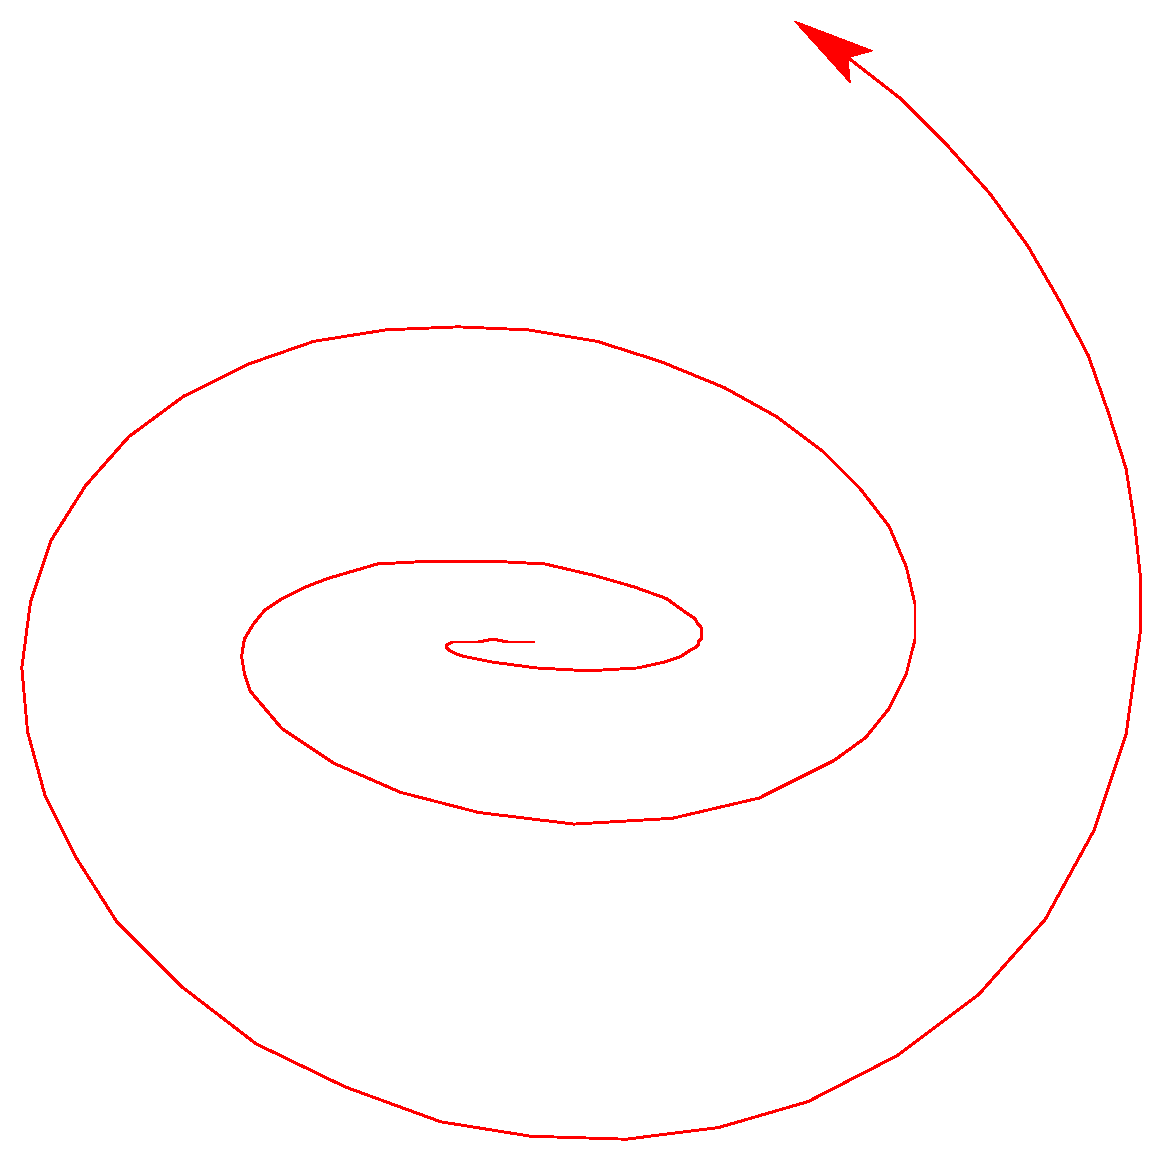
\includegraphics[width=6cm]{C6430_4.pdf}
 % C6430_3.pdf: 556x556 pixel, 72dpi, 19.61x19.61 cm, bb=0 0 556 556
\end{center}
\caption{branche infinie sans direction asymptotique}
\end{figure}

\begin{defi}[Asymptote]\index{asymptote}
 On dira que $f$ admet une branche infinie avec une droite asymptote $\mathcal D$ lorsque 
\begin{displaymath}
 \Vert \overrightarrow{Af(t)}\Vert \xrightarrow[t_0]{} +\infty 
\text{ et }
d(f(t),\mathcal D) \xrightarrow[t_0]{} 0
\end{displaymath}
\end{defi}
\begin{prop}
 Une courbe paramétrée $f$ admet une branche infinie avec une droite asymptote si et seulement si elle admet une directions asymptotique $\overrightarrow u$ et qu'il existe un point $A$ et un réel $l_A$ tel que
\begin{displaymath}
 \det(\overrightarrow{Af(t)},\overrightarrow u)\xrightarrow[t_0]{} l_A
\end{displaymath}
Dans ce cas, la droite asymptote est formée par les points $M$ tels que
\begin{displaymath}
 \det(\overrightarrow{Af(t)},\overrightarrow u)= l_A
\end{displaymath}
\end{prop}
\begin{demo}
  Vérifions que si on change de point, on change de limite $l_A$ mais pas de droite.
  Montrons que la distance de $f(t)$ à cette droite tends vers $0$.
\end{demo}
La proposition précédente conduit à une équation de l'asymptote et constitue une méthode pratique.\index{sf branches infinies}
\begin{exples}
\begin{enumerate}
 \item Courbes paramétrées $f(t)=O+u(t)\overrightarrow i +v(t)\overrightarrow j$ avec $u$ ou $v$ qui tend vers l'infini.à rédiger
 \item Cas d'une courbe en polaire : 
\begin{displaymath}
\left. 
\begin{aligned}
 f(\theta)=O+\rho(\theta)\overrightarrow{e}_{\theta}\\
\rho \xrightarrow[\theta_0]{} +\infty
\end{aligned}
\right\rbrace 
\Rightarrow \frac{1}{\Vert\overrightarrow{Of(\theta)} \Vert}\overrightarrow{Of(\theta)} = \overrightarrow{e}_{\theta} 
\xrightarrow[\theta_0]{} \overrightarrow{e}_{\theta_O}
\end{displaymath}
Il y a donc toujours une direction asymptotique. Il y a une asymptote si et seulement si le déterminant converge or
\begin{displaymath}
 \det(\overrightarrow{Of(\theta)},\overrightarrow{e}_{\theta_O}) = \rho(\theta)\sin(\theta - \theta_0)
\end{displaymath}
On obtient donc une forme indéterminée que l'on traite avec les outils de l'analyse. Lorsqu'il existe une limite finie $l$, on obtient une équation polaire de la droite asymptote qu'il est facile d'exprimer en coordonnées cartésiennes en développant simplement le $\sin$.
\begin{displaymath}
 \rho \sin(\theta -\theta_0) = l
\Leftrightarrow
-x\sin\theta_0 + y\cos\theta_0 = l
\end{displaymath}
\end{enumerate}
\end{exples}

\subsection{Calculs de vitesse}
\section{Exemples}
\begin{enumerate}
\item cardioïde\index{cardioïde}. Recherche des symétries, calcul vitesse, équation d'une tangente, tracé.
\begin{displaymath}
 f(\theta)= O +(1+\cos(\theta))\overrightarrow{e}_\theta
\end{displaymath}

 \item Recherche des symétries, tracé, équation cartésienne de la trajectoire
\begin{displaymath}
 f(t)= O+(t+\frac{1}{t})\overrightarrow{i} + (t^2+\frac{1}{t^2})\overrightarrow{j} 
\end{displaymath}

\item Recherche des points multiples, branches infinies
\begin{displaymath}
 f(t)= O+(t+\frac{2t}{t^2-1})\overrightarrow{i} + (\frac{(t+1)^2}{t^2})\overrightarrow{j} 
\end{displaymath}

\item Recherche des symétries, régionnement, branches infinies.
\begin{displaymath}
 f(\theta)= O +\dfrac{1}{2\cos\theta\cos(2\theta)}\overrightarrow{e}_\theta
\end{displaymath}
\end{enumerate}

\section{Savoir-faire}
\begin{enumerate}
 \item Tracé à la machine, syntaxe Maple de \verb|plot|. Sans machine, s'aider des autres points et former éventuellement des tableaux de variation.
\item Symétries. Trouver $S$ tel que $f(t')=S(f(t))$ où $S$ est une transformation du plan.
\item Régionnement attaché au signe de $\rho(\theta)$ pour une courbe polaire.
\item Calculs de vitesse comme pour la cardioïde.
\item \'Equations de tangentes et de normale.
\item Branches infinies.
\item \'Equations cartésiennnes point multiples. Ne pas manquer les équations des courbes polaires usuelles :
\begin{align*}
 \rho(\theta) =& a\cos\theta + b\sin \theta & & x^2+y^2 = ax +by \\
\rho(\theta) =& \dfrac{1}{a\cos\theta + b\sin \theta} & & 1=& ax +by
\end{align*}
en multipliant la premiere équation par $\rho$ et la deuxième par $a\cos \theta +b\sin\theta$.
\end{enumerate}

\end{document}
